\bigskip

\item Three different functions of the form $y = A \sin ( B x + C)$ are plotted below.  Could these all have the same value of $B$?

% \resizebox{3in}{!}{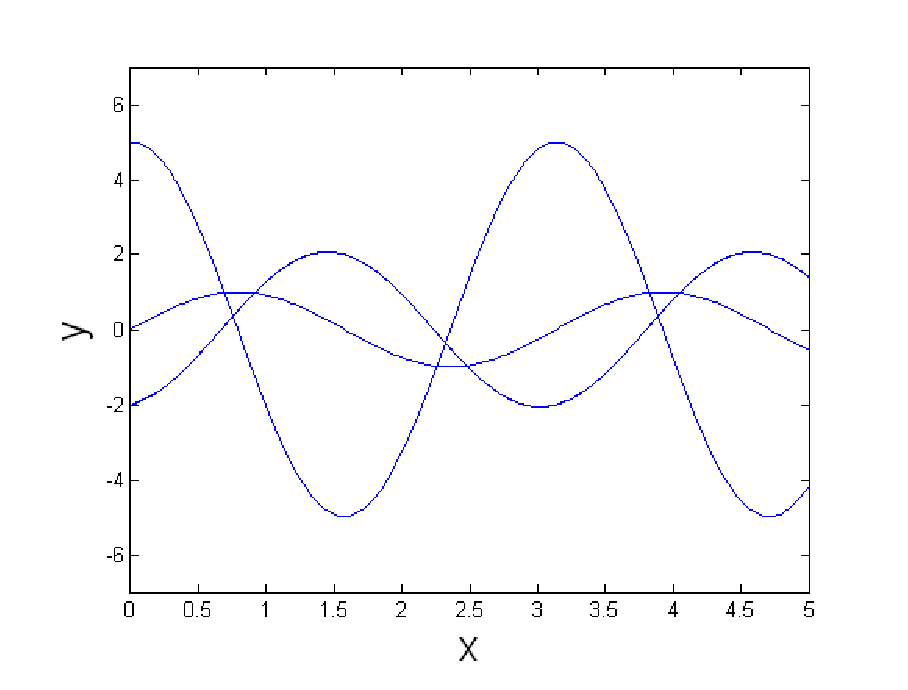
\includegraphics{SVC.01.05.060.ps}}

    \begin{minipage}{0.4\columnwidth}
        \begin{enumerate}
            \item Yes
            \item No
            \item Not enough information is given.
        \end{enumerate}
    \end{minipage}
\begin{minipage}{0.6\columnwidth}
    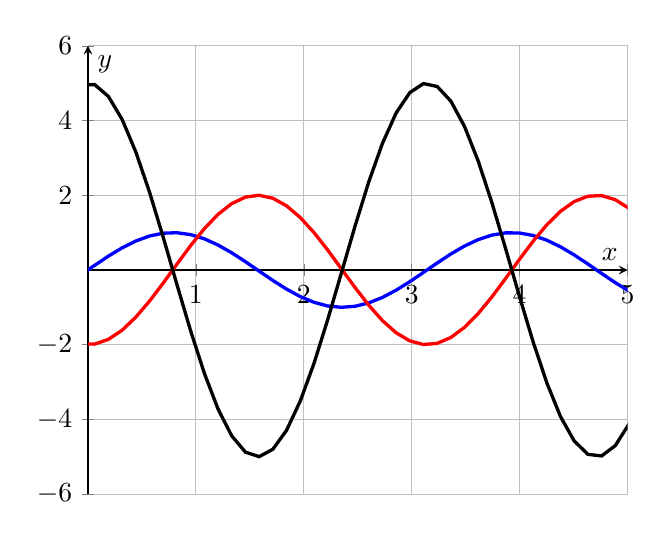
\begin{tikzpicture}
        \begin{axis}[axis lines=center, xlabel={$x$}, ylabel={$y$}, xmin=0, xmax=5,
                ymin=-6, ymax=6, grid]
                \addplot[color=blue, very thick,domain=-2*pi:2*pi, samples=100]
                {sin(deg(x)*2)};
                \addplot[color=red, very thick,domain=-2*pi:2*pi, samples=100]
                {-2*cos(deg(x)*2)};
                \addplot[color=black, very thick,domain=-2*pi:2*pi, samples=100]
                {5*cos(deg(x)*2)};
            \end{axis}
    \end{tikzpicture}
\end{minipage}



% Carroll College MathQuest

